\section{Footprinting}

\textbf{Footprinting} consists in someone doing passive(reconnaissance) or active(scanning) information gathering about some target. This enables an attacker to create a near complete profile of an organisation’s security posture. 

In our case, we will be Footprinting the following systems:

\subsection{137.74.187.100}

\subsubsection{Hacker Target - Reverse DNS \& nslookup}

Using the \href{https://hackertarget.com/reverse-dns-lookup/}{Reverse DNS Lookup} we were able to know to which domain this address belongs to: 

\begin{lstlisting}
    137.74.187.100 hackthissite.org
\end{lstlisting}

\begin{figure}[ht!]
 	\centering
 	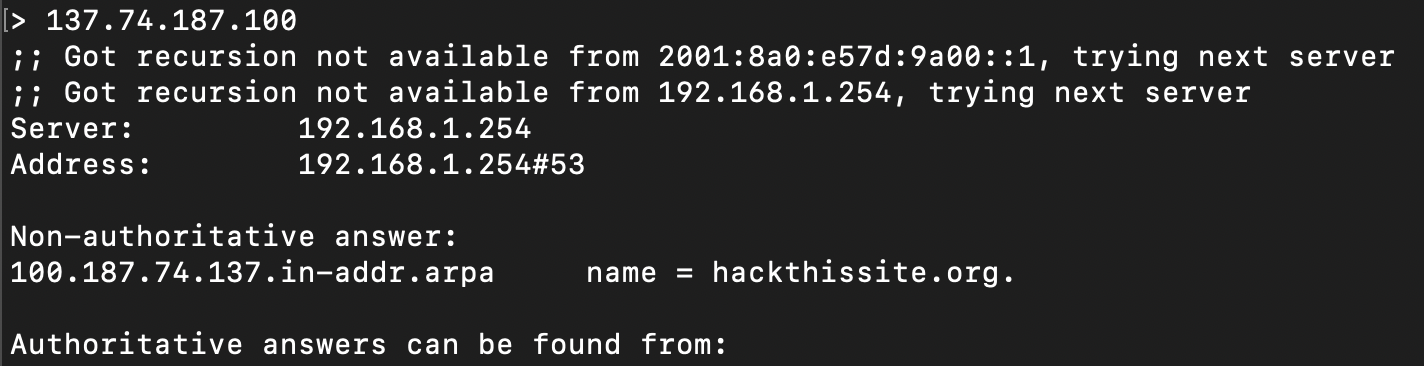
\includegraphics[width=1\linewidth]{img/nsl1.png}
 	\caption{nslookup result}
 \end{figure}

Using nslookup we were also able to perform a reverse dns search, obtaining a non-authoritative answer with the same result.

\subsubsection{dig}

Using dig, we can retrieve DNS records related to our targets IP address. By querying dig with our target it returns the following response:

\pagebreak

\begin{figure}[ht!]
 	\centering
 	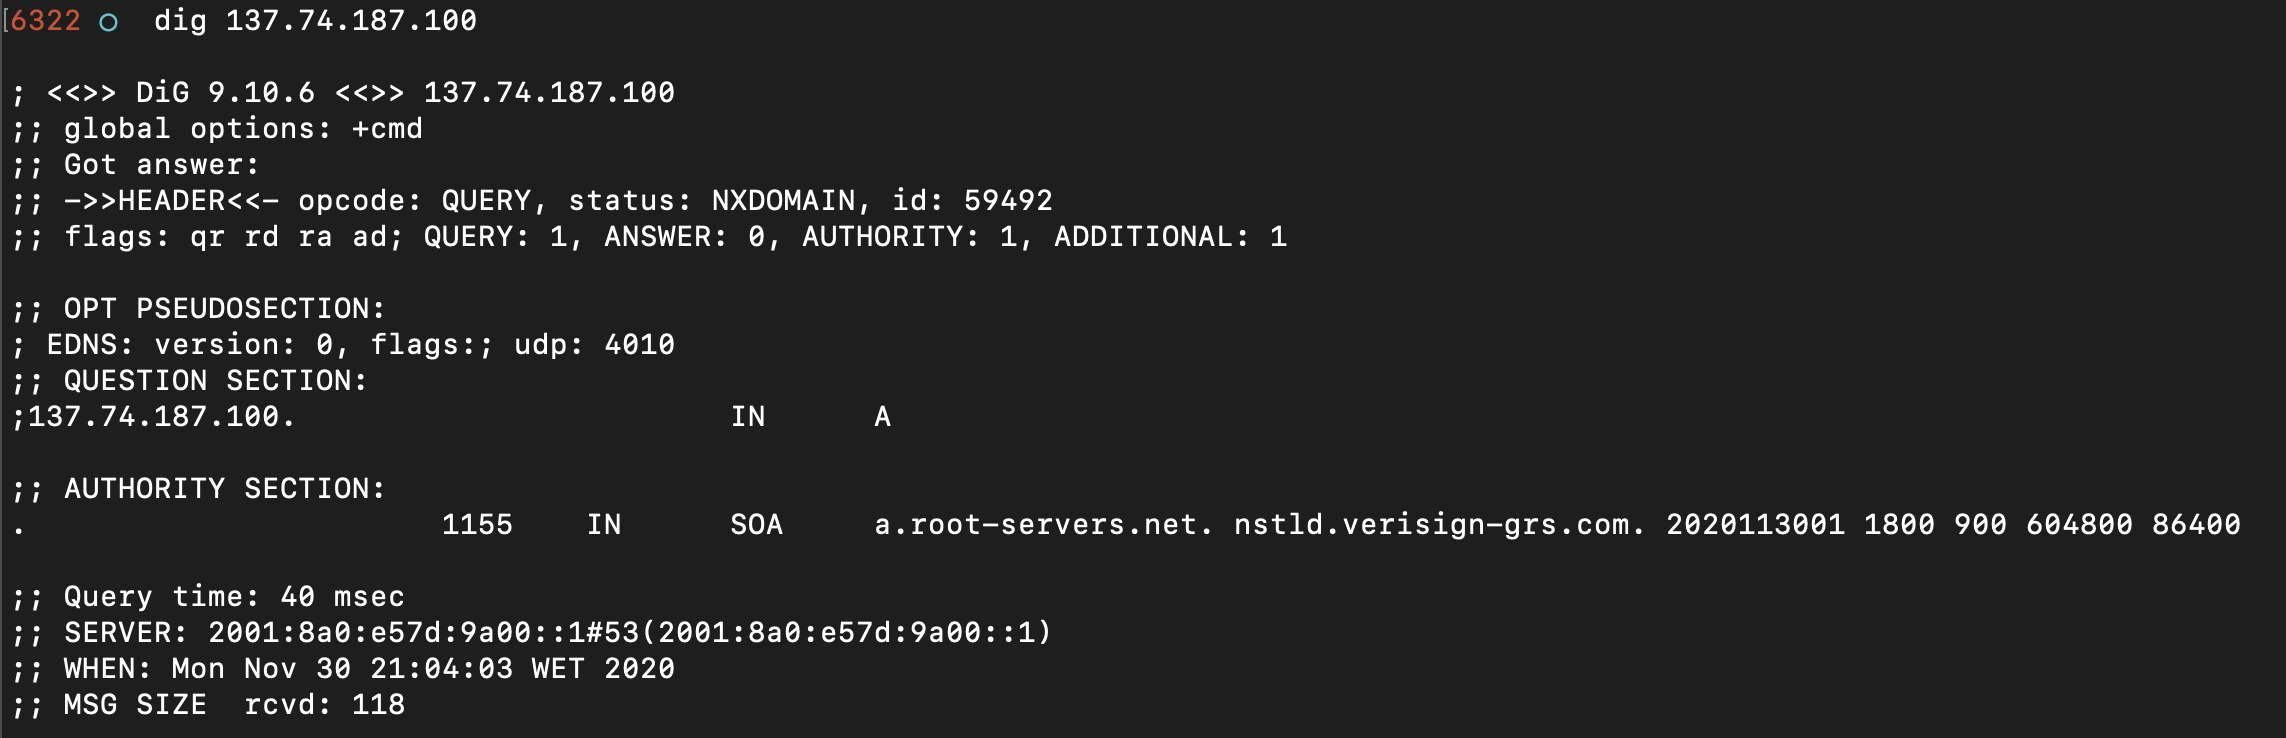
\includegraphics[width=1\linewidth]{img/dig1.png}
 	\caption{dig result}
 \end{figure}

In this case, we were able to retrieve a SOA record.

\subsubsection{IP2Location.com}

Using the \href{https://www.ip2location.com/demo}{IP2Location} tool we were able to know exactly where in the world this IP address is located and we can also get a lot of information about its ISP and its ASN number.

\begin{figure}[ht!]
 	\centering
 	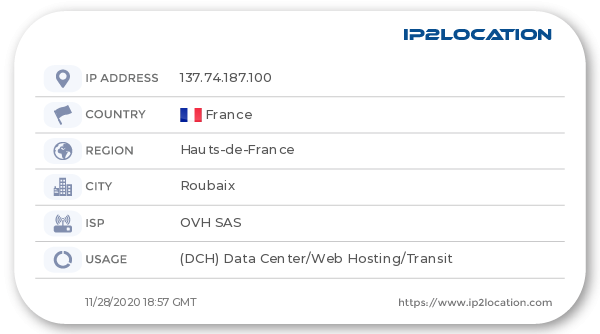
\includegraphics[width=0.7\linewidth]{img/ip2location137.png}
 	\caption{IP2Location result}
 \end{figure}
 
 
 Other information gathered includes:
 \begin{itemize}
    \item City Coordinates: 50°41'39"N   3°10'28"E
    \item Local Time: 28 Nov, 2020 07:55 PM (UTC +01:00)
    \item ZIP Code: 59689
    \item Elevation: 32m
    \item ASN: 16276 OVH
    \item Proxy Type: (DCH) Hosting Provider, Data Center or CDN Range
 \end{itemize}
 
\subsubsection{Spyse}

Using the \href{https://spyse.com/target/ip/137.74.187.100}{Spyse} tool we were able to discover open ports and technologies being used with related CVE's as well: 
 
 \begin{itemize}
    \item Open Ports: 80 (uses http protocol) and 443
    \item Technologies Used: jQuery Ver 1.8.1
 \end{itemize}
 
 There were listed 6 CVE, but the free tier only shows the first 4:
 \begin{itemize}
    \item CVE-2020-11022
    \item CVE-2020-11023
    \item CVE-2020-7656
    \item CVE-2012-6708
 \end{itemize}
 
 \subsubsection{nmap}

Using the nmap tool we were able to scan ports on the targeted IP, as well as seeing what service is using it. Nmap was only able of doing a guess about possible Operation Systems because the fingerprint wasn't ideal. The command for running nmap with OS detection (-O) and to use the TCP SYN technique (-sS) is:

\begin{lstlisting}
     nmap -v -sS -O 137.74.187.100
\end{lstlisting}

The report that nmap returned gave us information

\begin{lstlisting}
    Nmap scan report for hackthissite.org (137.74.187.100)
    Host is up (0.040s latency).
    Not shown: 997 filtered ports
    PORT    STATE  SERVICE
    22/tcp  closed ssh
    80/tcp  open   http
    443/tcp open   https

    Device type: bridge|general purpose
    Running (JUST GUESSING): Oracle Virtualbox (98%), QEMU (93%)
    OS CPE: cpe:/o:oracle:virtualbox cpe:/a:qemu:qemu
    Aggressive OS guesses: 
        - Oracle Virtualbox (98%), 
        - QEMU user mode network gateway (93%)
    No exact OS matches for host (test conditions non-ideal).
    TCP Sequence Prediction: Difficulty=17 (Good luck!)
    IP ID Sequence Generation: Incremental

\end{lstlisting}
 
\subsubsection{Shodan}

Using the \href{https://www.shodan.io/host/137.74.187.100}{Shodan} website we were able to scan ports as before and get information about the SSL certificate. The majority of information that Shodan retrieved we already had uncovered.
    

\subsection{216.58.215.148}

\subsubsection{Hacker Target - Reverse DNS \& nslookup}

Using the \href{https://hackertarget.com/reverse-dns-lookup/}{Reverse DNS Lookup} we were able to know to which domain this address belongs to: 

\begin{lstlisting}
    216.58.215.148 mad41s04-in-f20.1e100.net
\end{lstlisting}

\begin{figure}[ht!]
 	\centering
 	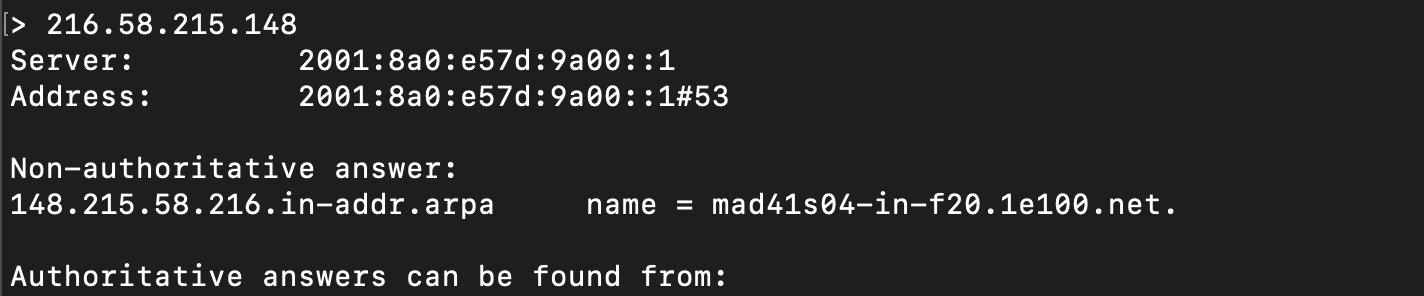
\includegraphics[width=1\linewidth]{img/nsl2.png}
 	\caption{nslookup result}
\end{figure}

Using nslookup we were also able to perform a reverse dns search, obtaining a non-authoritative answer with the same result.

\subsubsection{dig}

Using dig, we can retrieve DNS records related to our targets IP address. By querying dig with our target it returns the following response:

\begin{figure}[ht!]
 	\centering
 	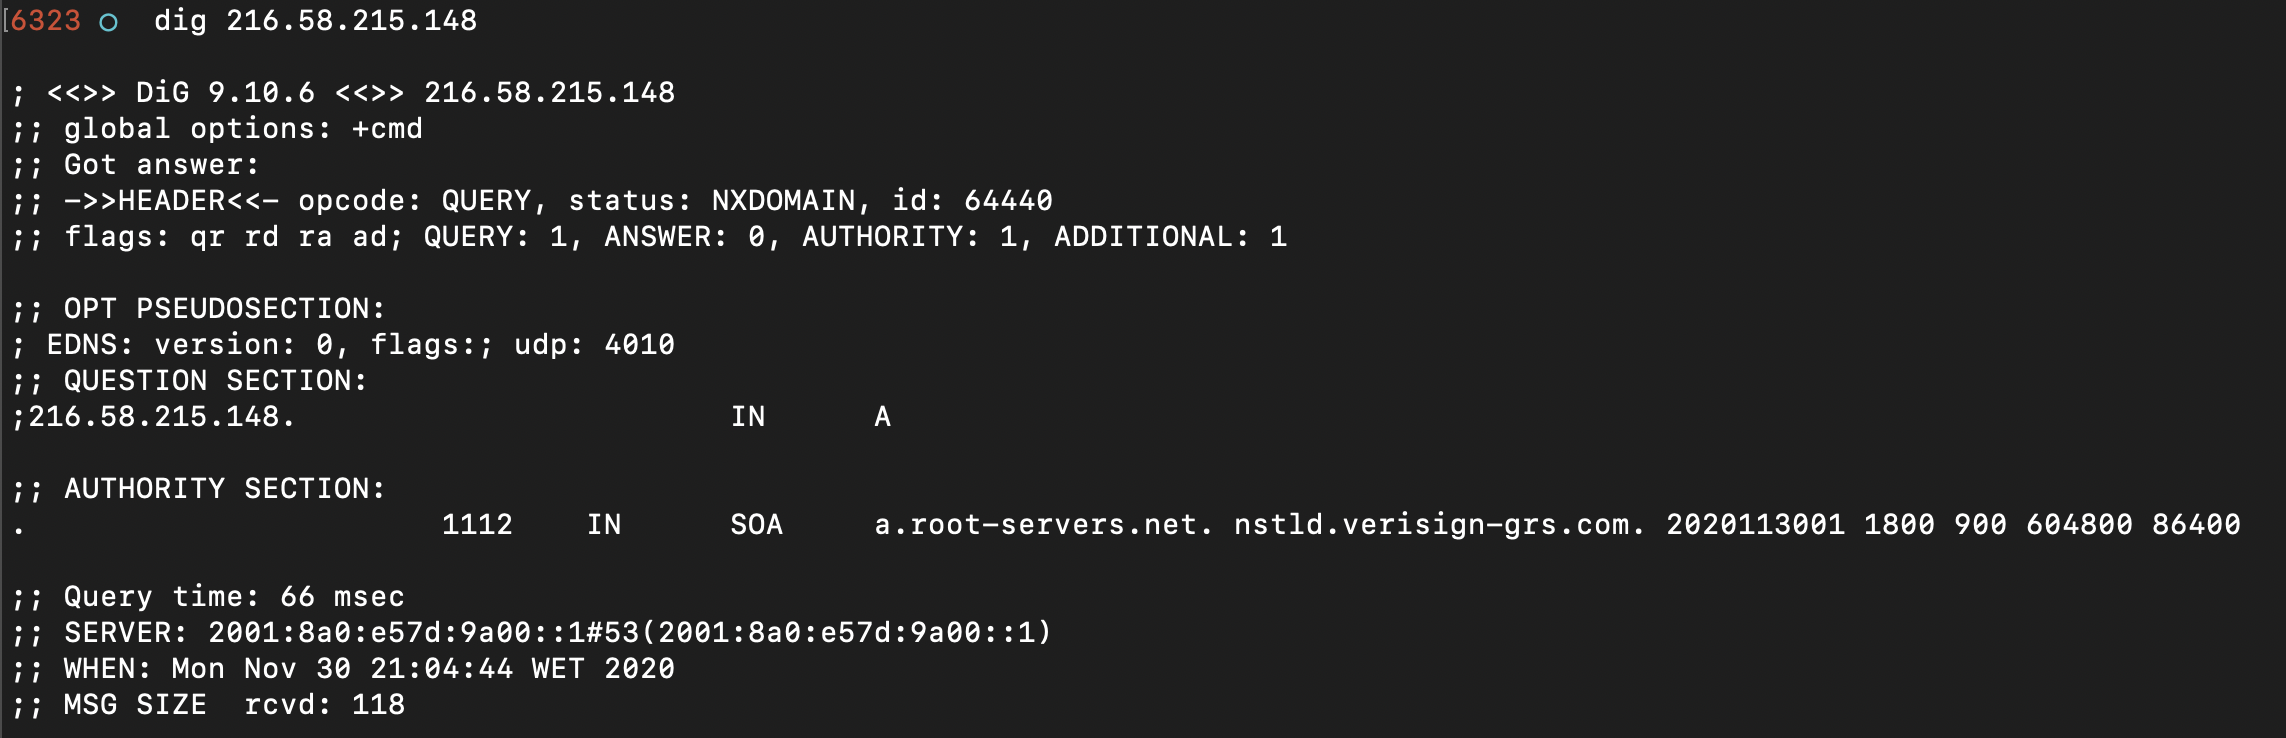
\includegraphics[width=1\linewidth]{img/dig2.png}
 	\caption{dig result}
 \end{figure}

In this case, we were able to retrieve a SOA record.

\subsubsection{IP2Location.com}

Using the \href{https://www.ip2location.com/demo}{IP2Location} tool we were able to know exactly where in the world this IP address is located and we can also get a lot of information about its ISP and its ASN number.

\begin{figure}[ht!]
 	\centering
 	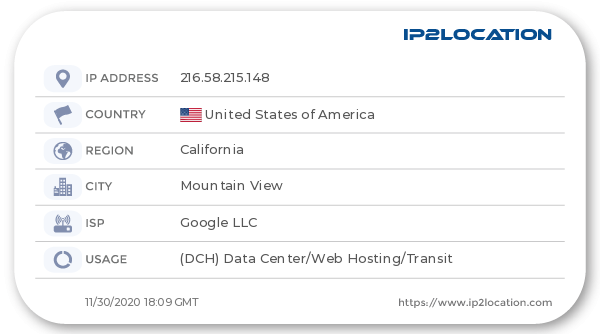
\includegraphics[width=0.6\linewidth]{img/ip2location216.png}
 	\caption{IP2Location result}
 \end{figure}
 
 \pagebreak
 
 Other information gathered includes:
 \begin{itemize}
    \item City Coordinates: 37°24'22"N   122°4'43"W
    \item Local 30 Nov, 2020 09:55 AM (UTC -08:00)
    \item ZIP Code: 94043
    \item Elevation: 32m
    \item ASN: 15169 Google
    \item Proxy Type: (DCH) Hosting Provider, Data Center or CDN Range
 \end{itemize}
 
\subsubsection{Spyse}

Using the \href{https://spyse.com/target/ip/216.58.215.148}{Spyse} tool we were able to discover only open ports, no technologies being used, nor CVE's: 
 
 \begin{itemize}
    \item Open Ports: 80 (uses http protocol) and 443
 \end{itemize}
 
This site couldn't find any vulnerabilities to the given IP. Awarding a Security Score of 100, meaning it has a low security risk.


\subsubsection{nmap}

Using the nmap tool we were able to scan ports on the targeted IP, as well as seeing what service is using it. This time, Nmap was able to obtain the Operation System. The command for running nmap with OS detection (-O) and to use the TCP SYN technique (-sS) is:

\begin{lstlisting}
     nmap -v -sS -O 216.58.215.14
\end{lstlisting}

The report that nmap returned gave us information

\begin{lstlisting}
    Nmap scan report for fra21s02-in-f14.1e100.net (216.58.215.14)
    Host is up (0.0055s latency).
    Not shown: 991 filtered ports
    PORT    STATE SERVICE
    25/tcp  open  smtp
    110/tcp open  pop3
    119/tcp open  nntp
    143/tcp open  imap
    465/tcp open  smtps
    563/tcp open  snews
    587/tcp open  submission
    993/tcp open  imaps
    995/tcp open  pop3s

    Device type: bridge
    Running: Oracle Virtualbox
    OS CPE: cpe:/o:oracle:virtualbox
    OS details: Oracle Virtualbox
    TCP Sequence Prediction: Difficulty=18 (Good luck!)
    IP ID Sequence Generation: Incremental
\end{lstlisting}
 
\subsubsection{Shodan}

Using the \href{https://www.shodan.io/host/216.58.215.148}{Shodan} website we were able to scan ports as before, get information about the SSL certificate. The majority of information that Shodan retrieved we already had uncovered.


\subsection{45.33.32.156}

\subsubsection{Hacker Target - Reverse DNS \& nslookup}

Using the \href{https://hackertarget.com/reverse-dns-lookup/}{Reverse DNS Lookup} we were able to know to which domain this address belongs to: 

\begin{lstlisting}
    45.33.32.156 scanme.nmap.org
\end{lstlisting}

\begin{figure}[ht!]
 	\centering
 	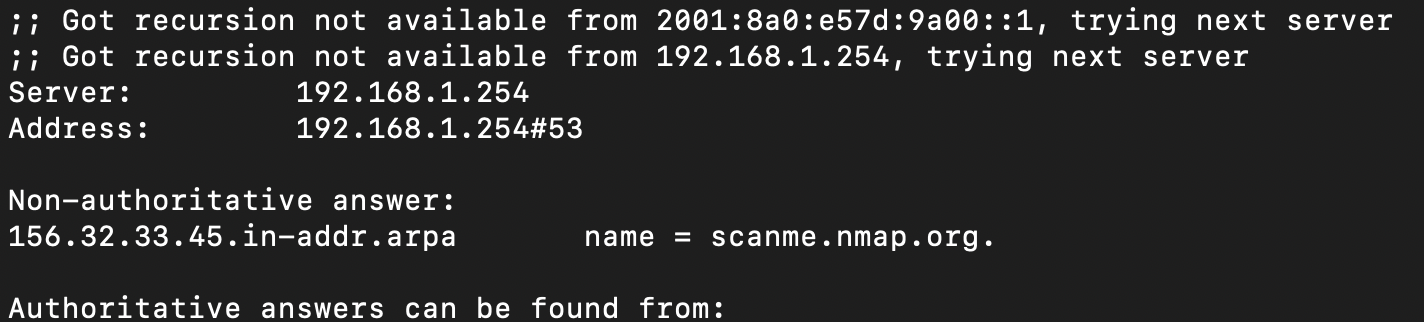
\includegraphics[width=1\linewidth]{img/nsl3.png}
 	\caption{nslookup result}
\end{figure}

Using nslookup we were also able to perform a reverse dns search, obtaining a non-authoritative answer with the same result.

\vspace{0.5cm}

\subsubsection{dig}

Using dig, we can retrieve DNS records related to our targets IP address. By querying dig with our target it returns the following response:

\begin{figure}[ht!]
 	\centering
 	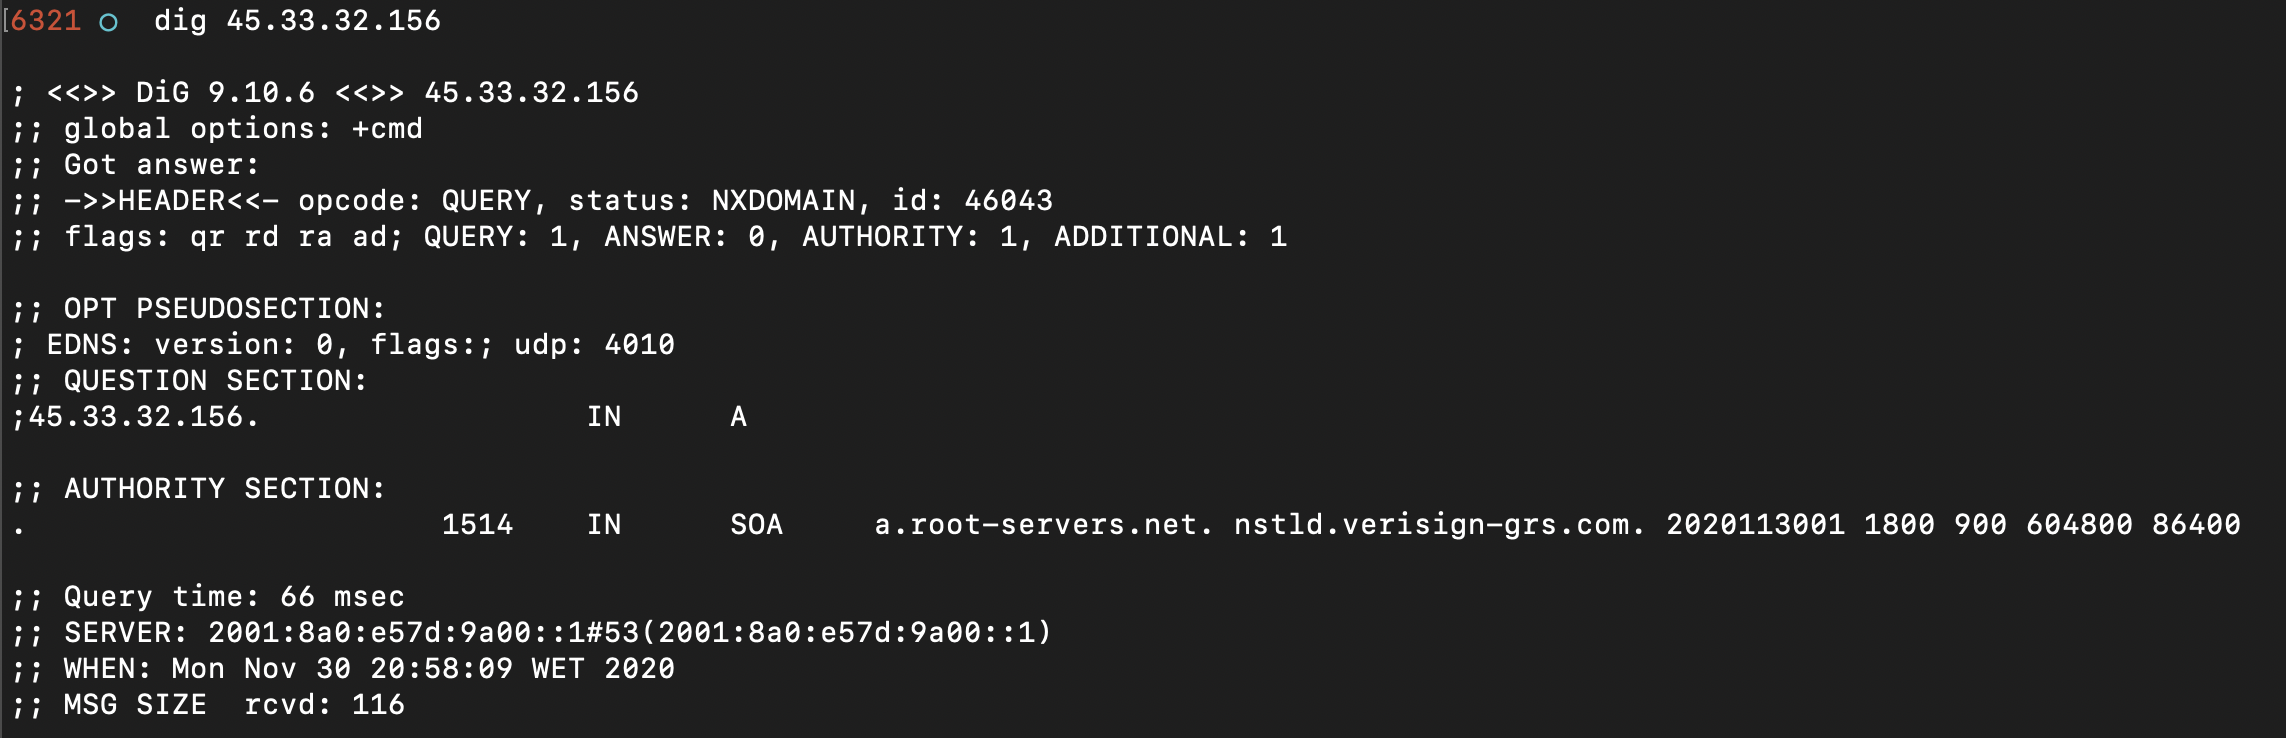
\includegraphics[width=1\linewidth]{img/dig3.png}
 	\caption{dig result}
 \end{figure}

In this case, we were able to retrieve a SOA record.

\vspace{0.5cm}

\subsubsection{IP2Location.com}

Using the \href{https://www.ip2location.com/demo}{IP2Location} tool we were able to know exactly where in the world this IP address is located and we can also get a lot of information about its ISP and its ASN number.

\vspace{3cm}

\begin{figure}[ht!]
 	\centering
 	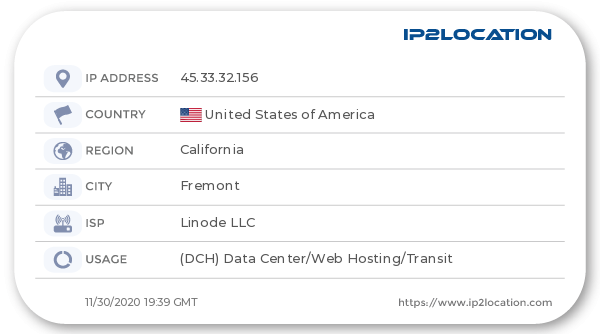
\includegraphics[width=0.7\linewidth]{img/ip2location45.png}
 	\caption{IP2Location result}
 \end{figure}

Other information gathered includes:
 \begin{itemize}
    \item City Coordinates: 37°32'54"N    121°59'19"W
    \item Local Time: 30 Nov, 2020 11:15 AM (UTC -08:00)
    \item ZIP Code: 94536
    \item Elevation: 16m
    \item ASN: 63949 Linode LLC
    \item Proxy Type: (VPN) VPN Server
 \end{itemize}

\subsubsection{Spyse}

Using the \href{https://spyse.com/target/ip/45.33.32.156}{Spyse} tool we were able to discover open ports and technologies being used with related CVE's as well: 
 
 \begin{itemize}
    \item Open Ports: 80 (uses http protocol) and 22
    \item Technologies Used: Google AdSense, OpenSSH Ver 6.6.1p1 and Apache Ver 2.4.7  
 \end{itemize}
 
 There were listed 6 CVE, but the free tier only shows the first 4:
 \begin{itemize}
    \item CVE-2019-0217
    \item CVE-2016-2161
    \item CVE-2015-8325
    \item CVE-2016-3115
 \end{itemize}
 
 We were also able to see the Banners on ports 80 and 22:
 
 \begin{lstlisting}
Port 80:
    HTTP/1.1 200 OK
    Date: Tue, 03 Nov 2020 21:30:32 GMT
    Server: Apache/2.4.7 (Ubuntu)
    Accept-Ranges: bytes
    Vary: Accept-Encoding
    Connection: close
    Content-Type: text/html

Port 22: 
    SSH-2.0-OpenSSH_6.6.1p1 Ubuntu-2ubuntu2.13
 \end{lstlisting}
 
\subsubsection{nmap}

Using the nmap tool we were able to scan ports on the targeted IP, as well as seeing what service is using it. Just like the first IP address, nmap was only able of doing a guess about possible Operation Systems, because the fingerprint wasn't ideal. The command for running nmap with OS detection (-O) and to use the TCP SYN technique (-sS) is:

\begin{lstlisting}
     nmap -v -sS -O 45.33.32.156
\end{lstlisting}

The report that nmap returned gave us information

\begin{lstlisting}
    Nmap scan report for scanme.nmap.org (45.33.32.156)
    Host is up (0.17s latency).
    Not shown: 996 closed ports
    PORT      STATE SERVICE
    22/tcp    open  ssh
    80/tcp    open  http
    9929/tcp  open  nping-echo
    31337/tcp open  Elite
    Aggressive OS guesses: Linux 5.0 - 5.4 (96%), Linux 5.4 (95%), Linux 4.15 - 5.6 (94%), Linux 5.0 - 5.3 (93%), Linux 5.1 (93%), Linux 2.6.32 - 3.13 (93%), Linux 5.0 (92%), Linux 2.6.22 - 2.6.36 (91%), Linux 3.10 - 4.11 (91%), Linux 3.10 (91%)
    No exact OS matches for host (test conditions non-ideal).
    Uptime guess: 15.079 days (since Sun Nov 15 18:01:15 2020)
    Network Distance: 20 hops
    TCP Sequence Prediction: Difficulty=264 (Good luck!)
    IP ID Sequence Generation: All zeros
\end{lstlisting}

Using nmap we discovered 2 new open ports and we use it's OS prediction to have a slight idea of the targets OS type(Linux).
 
\subsubsection{Shodan}

Using the \href{https://www.shodan.io/host/45.33.32.156}{Shodan} website we were able to scan ports as before, including a new one (port 123), get information about the OpenSSH, and we discovered a lot of CVE's. The majority of information that Shodan retrieved we already had uncovered.
    

\pagebreak